\documentclass[lang=cn,10pt]{elegantbook}
\usepackage{xcolor} % 用于颜色定义
\usepackage{listings} % 用于代码高亮
\usepackage[UTF8]{ctex} % 引入 ctex 宏包以支持中文
\usepackage{graphicx}

\lstset{
    language=C++, % 代码语言
    basicstyle=\ttfamily, % 使用等宽字体
    keywordstyle=\color{black}, % 关键词颜色
    commentstyle=\color{black}, % 注释颜色
    stringstyle=\color{black}, % 字符串颜色
    breaklines=true, % 自动换行
    numbers=left, % 行号在左侧显示
    numberstyle=\tiny, % 行号字体大小
    frame=single, % 代码框样式
    showstringspaces=false, % 不显示字符串中的空格标记
}

\title{操作系统}
\subtitle{YuTeng\LaTeX{}}

\author{Yu Teng}
\institute{和光同尘}
\date{December 29, 2024}
\version{1.0}

\extrainfo{不要以为抹消过去,重新来过,即可发生什么改变。—— 比企谷八幡}

\setcounter{tocdepth}{3}

\logo{logo-blue.png}
\cover{cover.jpg}

% 本文档命令
\usepackage{array}
\newcommand{\ccr}[1]{\makecell{{\color{#1}\rule{1cm}{1cm}}}}


\begin{document}

\maketitle
\frontmatter

\tableofcontents

\mainmatter

\chapter{计算机系统概述}

\section{}

\subsection{}


\chapter{进程与线程}

\section{进程与线程}

\section{CPU调度}

\section{同步与互斥}

\subsection{经典同步问题}

【生产者-消费者问题】一组生产者进程和一组消费者进程共享一个初始为空、大小为n的缓冲区。只有当缓冲区不满时,生产者才能将消息放入缓冲区;否则必须阻塞,
等待消费者从缓冲区中取出消息后将其唤醒。只有当缓冲区不空时,消费者才能从缓冲区中取出消息;否则必须等待,等待生产者将消息放入缓冲区后将其唤醒。
由于缓冲区是临界资源,因此必须互斥访问。

分析:

1)关系分析。生产者和消费者对缓冲区互斥访问是互斥关系,同时生产者和消费者又是一个相互协作的关系,只有生产者生产之后,消费者才能消费,它们也是同步关系。

2)整理思路。这里比较简单,只有生产者和消费者两个进程,正好是这两个进程存在着互斥关系和同步关系。那么需要解决的是互斥和同步PV操作的位置。

3)信号量设置。信号量 mutex 作为互斥信号量,用于控制互斥访问缓冲池,互斥信号量初值为 1;信号量full用于记录当前缓冲池中的“满”缓冲区数,初值为 0。信号量 empty用于记录当前缓冲池中的“空”缓冲区数,初值为 n。

问题解答:

\begin{lstlisting}
    semaphore mutex=1,empty=N,full=0;  // mutex互斥信号量用于互斥使用缓冲区,empty,full同步信号量只有缓冲区有空闲生产者才能放,只有缓冲区有资源消费者才能取。
    P1() { // 生产者进程
        while(1) {
            生产一个资源
            P(empty); // 缓冲区是否有空闲,消耗一个空闲位置
            P(mutex);  // 互斥使用缓冲区
            将一个资源放入缓冲区
            V(mutex); // 归还缓冲区使用权
            V(full); // 缓冲区资源数加1,唤醒消费者进程
        }
    }
    P2() { // 消费者进程
        while(1) {
            P(full); //有资源时候被唤醒
            P(mutex); // 互斥使用缓冲区
            从缓冲区中取出一个资源
            V(mutex); // 归还缓冲区使用权
            使用资源
        }
    }
\end{lstlisting}

【一个较为复杂的生产者-消费者问题】桌子上有一个盘子,每次只能向其中放入一个水果。爸爸专向盘子中放苹果,妈妈专向盘子中放橘子,儿子专等吃盘子中的橘子,女儿专等吃盘子中的苹果。只有盘子为空时,爸爸或妈妈才可向盘子中放一个水果:仅当盘子中有自己需要的水果时,儿子或女儿可以从盘子中取出。

分析:

问题解答:

\begin{lstlisting}
    semaphore mutex=1,empty=1,num_apple=0,num_orange=0;
    P1() { // 爸爸
        while(1) {
            P(empty);
            P(mutex); // 竞争盘子的使用权
            向盘子中放入一个苹果
            V(mutex); // 归还盘子的使用权
            V(num_apple); // 生产一个苹果
        }
    }
    P2(){ // 妈妈
        while(1) {
            P(empty);
            P(mutex); // 竞争盘子的使用权
            向盘子中放入一个橘子
            V(mutex); // 归还盘子的使用权
            V(num_orange); // 生产一个橘子
        }
    } 
    P3(){ // 儿子
        while(1) {
            P(num_orange);
            P(mutex);
            从盘子中拿走一个橘子
            V(mutex);
            V(empty);
        }
    }
    P4(){ // 女儿
        while(1) {
            P(num_apple);
            P(mutex);
            从盘子中拿走一个苹果
            V(mutex);
            V(empty);
        }
    }
\end{lstlisting}

注意这题和上面题的特殊性这里盘子里面只能放入一个水果,所以我们可以不需要使用mutex对盘子进行互斥使用,所以修改下面的代码如下。

\begin{lstlisting}
    semaphore empty=1,num_apple=0,num_orange=0;
    P1() { // 爸爸
        while(1) {
            P(empty);
            向盘子中放入一个苹果
            V(num_apple); // 生产一个苹果
        }
    }
    P2(){ // 妈妈
        while(1) {
            P(empty);
            向盘子中放入一个橘子
            V(num_orange); // 生产一个橘子
        }
    } 
    P3(){ // 儿子
        while(1) {
            P(num_orange);
            从盘子中拿走一个橘子
            V(empty);
        }
    }
    P4(){ // 女儿
        while(1) {
            P(num_apple);
            从盘子中拿走一个苹果
            V(empty);
        }
    }
\end{lstlisting}

【读者写者问题】有读者和写者两组并发进程,共享一个文件,当两个或以上的读进程同时访问共享数据时不会产生副作用,但若某个写进程和其他进程(读进程或写进程)同时访问共享数据时则可能导致数据不一致的错误。因此要求:(1)允许多个读者可以同时对文件执行读操作;(2)只允许一个写者往文件中写信息;(3)任意一个写者在完成写操作之前不允许其他读者或写者工作;(4)写者执行写操作前,应让已有的读者和写者全部退出。

\begin{lstlisting}
    int count=0; // 记录当前读者数量
    semaphore rw=1,mutex=1; // rw保证读写进程互斥 mutex保护count变量的更新
    P1() { // 写者进程
        while(1) {
            P(rw); // 互斥访问共享文件
            写文件
            V(rw); // 释放共享文件
        }
    }
    P2() { //读者进程
        while(1) {
            P(mutex); // 互斥访问count变量
            if(count==0) // 第一个读进程才需要rw锁,这样就可以使可以同时有多个读者读取文件
                P(rw); // 阻止写进程写
            count++; // 读者计数器+1
            V(mutex); // 释放互斥变量count
            读文件
            P(mutex); // 互斥访问count变量
            count--; // 读者计数器-1
            if(count==0) // 由最后一个读进程负责读完了解锁
                V(rw); // 允许写进程写
            V(mutex); // 释放互斥变量count
        }
    }

\end{lstlisting}

在上面的算法中,读进程是优先的,即当存在读进程时,写操作将被延迟,且只要有一个读进程活跃,随后而来的读进程都将被允许访问文件。这样的方式会导致写进程可能长时间等待,且存在写进程“饿死”的情况。

若希望写进程优先,即当有读进程正在读共享文件时,有写进程请求访问,这时应禁止后续读进程的请求,等到已在共享文件的读进程执行完毕,立即让写进程执行,只有在无写进程执行的情况下才允许读进程再次运行。为此,增加一个信号量并在上面程序的 writer()和 reader()函数中各增加一对 PV操作,就可以得到写进程优先的解决程序。

\begin{lstlisting}
    int count=0; // 记录当前读者数量
    semaphore rw=1,mutex=1,w=1; // rw保证读写进程互斥 mutex保护count变量的更新 w用于实现写优先
    P1() { // 写者进程
        while(1) {
            P(w);
            P(rw); // 互斥访问共享文件
            写文件
            V(rw); // 释放共享文件
            V(w);
        }
    }
    P2() { //读者进程
        while(1) {
            P(w);
            P(mutex); // 互斥访问count变量
            if(count==0) // 第一个读进程才需要rw锁,这样就可以使可以同时有多个读者读取文件
                P(rw); // 阻止写进程写
            count++; // 读者计数器+1
            V(mutex); // 释放互斥变量count
            V(w);
            读文件
            P(mutex); // 互斥访问count变量
            count--; // 读者计数器-1
            if(count==0) // 由最后一个读进程负责读完了解锁
                V(rw); // 允许写进程写
            V(mutex); // 释放互斥变量count
        }
    }
\end{lstlisting}

    上面这种写法可以实现写预先,让我们看一下下面几种情况时P(w),V(w)会如何保证写进程优先。

    (1) 读者1->读者2

    (2) 写者1->写者2

    (3) 写者1->读者1

    (4) 读者1->写者1->读者2

    (5) 写者1->读者1->写者2

【哲学家进餐问题】一张圆桌边上坐着5名哲学家,每两名哲学家之间的桌上摆一根筷子,两根筷子中间是一碗米饭,如图所示。哲学家们倾注毕生精力用于思考和进餐,哲学家在思考时,并不影响他人。只有当哲学家饥饿时,才试图拿起左、右两根筷子(一根一根地拿起)。若筷子已在他人手上,则需要等待。饥饿的哲学家只有同时拿到了两根筷子才可以开始进餐,进餐完毕后,放下筷子继续思考。

\begin{figure}[h]
    \centering
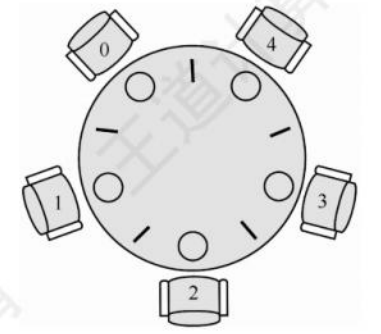
\includegraphics[width=0.3\textwidth]{image/哲学家进餐问题.png}
\end{figure}

分析:1)关系分析。5名哲学家与左右邻居对其中间筷子的访问是互斥关系。

2)整理思路。显然,这里有5个进程。本题的关键是如何让一名哲学家拿到左右两根筷子而不造成死锁或饥饿现象。解决方法有两个:一是让他们同时拿两根筷子:二是对每名哲学家的动作制定规则,避免饥饿或死锁现象的发生。

3)信号量设置。定义互斥信号量数组 chopstick[5]=\{1,1,1,1,1\},用于对5个筷子的互斥访问。哲学家按顺序编号为$0 \sim 4$,哲学家i左边筷子的编号为i,哲学家右边筷子的编号为(i+ 1)\%5 。

\subsection{历年真题解析}

    【2009真题】三个进程$P_1$、$P_2$、$P_3$互斥使用一个包含N(N$>$0)个单元的缓冲区。$P_1$每次用produce()生成一个正整数并用put()送入缓冲区某一空单元中;$P_2$每次用getodd()从该缓冲区中取出一个奇函数
    并用countodd()统计奇数个数;$P_3$每次用geteven()从该缓冲区中取出一个偶数并用counteven()统计偶数个数。请用信号量机制实现这三个进程的同步与互斥活动,并说明所定义信号量的含义(要求使用伪代码描述)。
    
    分析:有一个互斥使用的资源缓冲区三个进程互斥使用,有三个资源实现同步操作,缓冲区对于$P_1$需要有空闲位置才能放,而$P_2$,$P_3$需要缓冲区有奇数或者偶数才能被唤醒。
    
    答:
    \begin{lstlisting}
        semaphore mutex=1,empty=N,odd=0,even=0;  
        P1() { 
            while(1) {
                num = produce(); // 生成一个正整数,
                P(empty); // 缓冲区是否有空闲,消耗一个空闲位置
                P(mutex);  // 互斥使用缓冲区
                put(); // 就正整数放入缓冲区
                V(mutex); // 归还缓冲区使用权
                if(num%2==1)  
                    V(odd); // 生成奇数唤醒P2()
                else
                    V(even); // 生成偶数唤醒P3()
            }
        }
        P2() {
            while(1) {
                P(odd); //如果是奇数被唤醒
                P(mutex);
                getodd(); // 从缓冲区中取出一个奇数
                V(mutex); // 归还缓冲区使用权
                countodd(); //统计奇数个数
            }
        }
        P3() {
            while(1) {
                P(even); //如果是奇数被唤醒
                P(mutex);
                geteven(); // 从缓冲区中取出一个偶数
                V(mutex); // 归还缓冲区使用权
                counteven(); //统计偶数个数
            }
        }
    \end{lstlisting}

\section{死锁}









\end{document}
